%!TEX root = Slic3r-Manual.tex

There are two ways in which to organize the configuration settings: exporting and importing the configuration settings, and profiles.  The former is available in both simple and expert mode, whereas profiles is only available in expert mode.

\subsection{Exporting and Importing Configuration} % (fold)
\label{sub:exporting_and_importing_configuration}
\index{configuration!export}
\index{configuration!import}

The current set of configuration options can be simply exported via the \texttt{Export Config} File menu option. This saves all the values into a text file with a \texttt{.ini} extension.  Previously saved files can be loaded with the \texttt{Load Config} menu option.

This gives a rudimentary means to store different configuration settings for different needs.  For example a set with slightly faster print speeds, or a different infill pattern.  However this way of organizing things will quickly become frustrating, as each minor change to a parameter may have to be duplicated across many configurations.  For this reason, profiles are a more suitable way of managing multiple configurations.

This method also allows configuration to be transferred between machines, or stored remotely.

% subsection exporting_and_importing_configuration (end)


\subsection{Profiles} % (fold)
\label{sec:profiles}
\index{profiles}

After a few prints it will become apparent that it is worth having a set of configuration options to choose from, and that some parameters change at different rates as others.  In expert mode, profiles can be created for Print, Filament and Printer settings, with the expectation that the printer settings change least often, filament rarely, and the print settings could be changed for each model.  These different profiles can be mixed and matched as desired, and can be selected either in their respective tabs, or directly from the plater.

\subsubsection{Creating Profiles} % (fold)
\label{sub:creating_profiles}
\index{profiles!create}

Open the desired tab and change the settings as necessary.  Once satisfied, click the save icon to the left above the setting titles, and give a suitable name when prompted.

\begin{figure}[H]
\centering
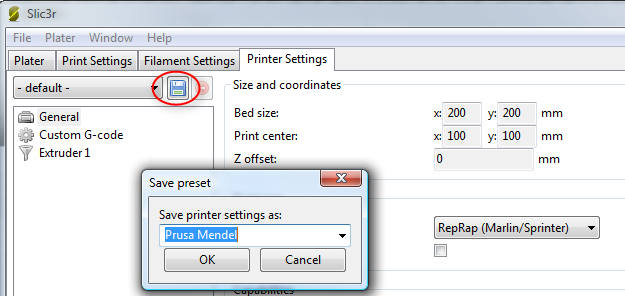
\includegraphics[keepaspectratio=true,width=1\textwidth]{organising/creating_a_profile.png}
\caption{Saving a profile.}
\label{fig:creating_a_profile}
\end{figure}

\index{profiles!delete}
Profiles can be deleted by choosing the profile to delete and clicking the red delete button next to the save button.

\begin{figure}[H]
\centering
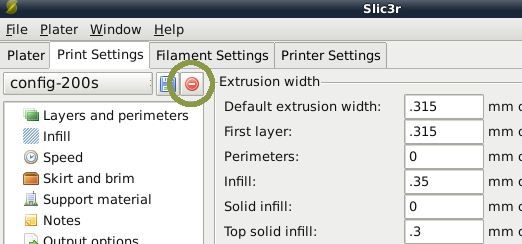
\includegraphics[keepaspectratio=true,width=1\textwidth]{organising/deleting_a_profile.png}
\caption{Deleting a profile.}
\label{fig:deleting_a_profile}
\end{figure}

% subsubsection creating_profiles (end)


% subsection profiles (end)
